\documentclass[conference]{IEEEtran}

% Pacotes para suporte ao Português e imagens
\usepackage[utf8]{inputenc}
\usepackage[T1]{fontenc}
\usepackage[brazilian]{babel}
\usepackage{amsmath,amssymb,amsfonts}
\usepackage{algorithmic}
\usepackage{graphicx}
\usepackage{textcomp}
\usepackage{xcolor}

\begin{document}

\title{Relatório de Práticas em Sistemas Digitais - Laboratórios 01 e 02}

\author{\IEEEauthorblockN{Lucca Pedreira Dultra, João Vital, Danyel}
\IEEEauthorblockA{\textit{Departamento de Computação (DCOMP)} \\
\textit{Universidade Federal de Sergipe (UFS)}\\
São Cristóvão, Brasil \\
}
}

\maketitle

\begin{abstract}
Este relatório descreve as atividades práticas conjuntas realizadas nos Laboratórios 01 e 02[cite: 1050, 1080]. A primeira parte foca na operação de instrumentos de bancada e na análise da dinâmica temporal de circuitos Resistor/Capacitor (RC), avaliando efeitos de carga e limites de frequência[cite: 1051, 1052]. A segunda parte aborda a compreensão e comparação estrutural entre as famílias lógicas TTL e CMOS, incluindo a leitura de datasheets e a montagem de inversores lógicos[cite: 1081, 1082]. O estudo estabelece a relação entre as limitações analógicas temporais e a implementação física das portas lógicas digitais.
\end{abstract}

\begin{IEEEkeywords}
Sistemas Digitais, Instrumentação, Circuito RC, CMOS, TTL, Inversores, Datasheet.
\end{IEEEkeywords}

% ==========================================
% LABORATÓRIO 01
% ==========================================
\section{Laboratório 01: Instrumentação e Circuito RC}

\subsection{Introdução Teórica}
Os sistemas digitais manipulam grandezas de forma discreta, permitindo decisões lógicas precisas, embora o hardware resida no mundo analógico[cite: 1053, 1055]. Para compreender limitações como atrasos de sinal, analisa-se o comportamento de capacitores em malhas RC[cite: 1056]. A tecnologia CMOS destaca-se pelo consumo estático quase nulo, consumindo energia significativamente apenas durante o chaveamento das capacitâncias[cite: 1057].

\subsection{Materiais Utilizados}
\begin{itemize}
    \item \textbf{Instrumentos:} Protoboard, multímetro, osciloscópio, gerador de funções e fonte de tensão[cite: 1058].
    \item \textbf{Componentes:} Fios, LEDs, resistores e capacitores (2.2 pF, 10 nF e 100 nF)[cite: 1059, 1060].
\end{itemize}

\subsection{Descrição das Atividades e Resultados}

\subsubsection{Instrumentação e Adaptação à Protoboard}
A atividade consistiu na montagem de um circuito simples com LED para adaptação ao manuseio da protoboard[cite: 1060]. Conforme ilustrado na Fig. 1, a correta alimentação do circuito resultou no acionamento do componente. A medição prévia do resistor revelou variações percentuais em relação ao valor nominal, confirmando as imperfeições do mundo físico real[cite: 1061, 1062].

\begin{figure}[htbp]
\centerline{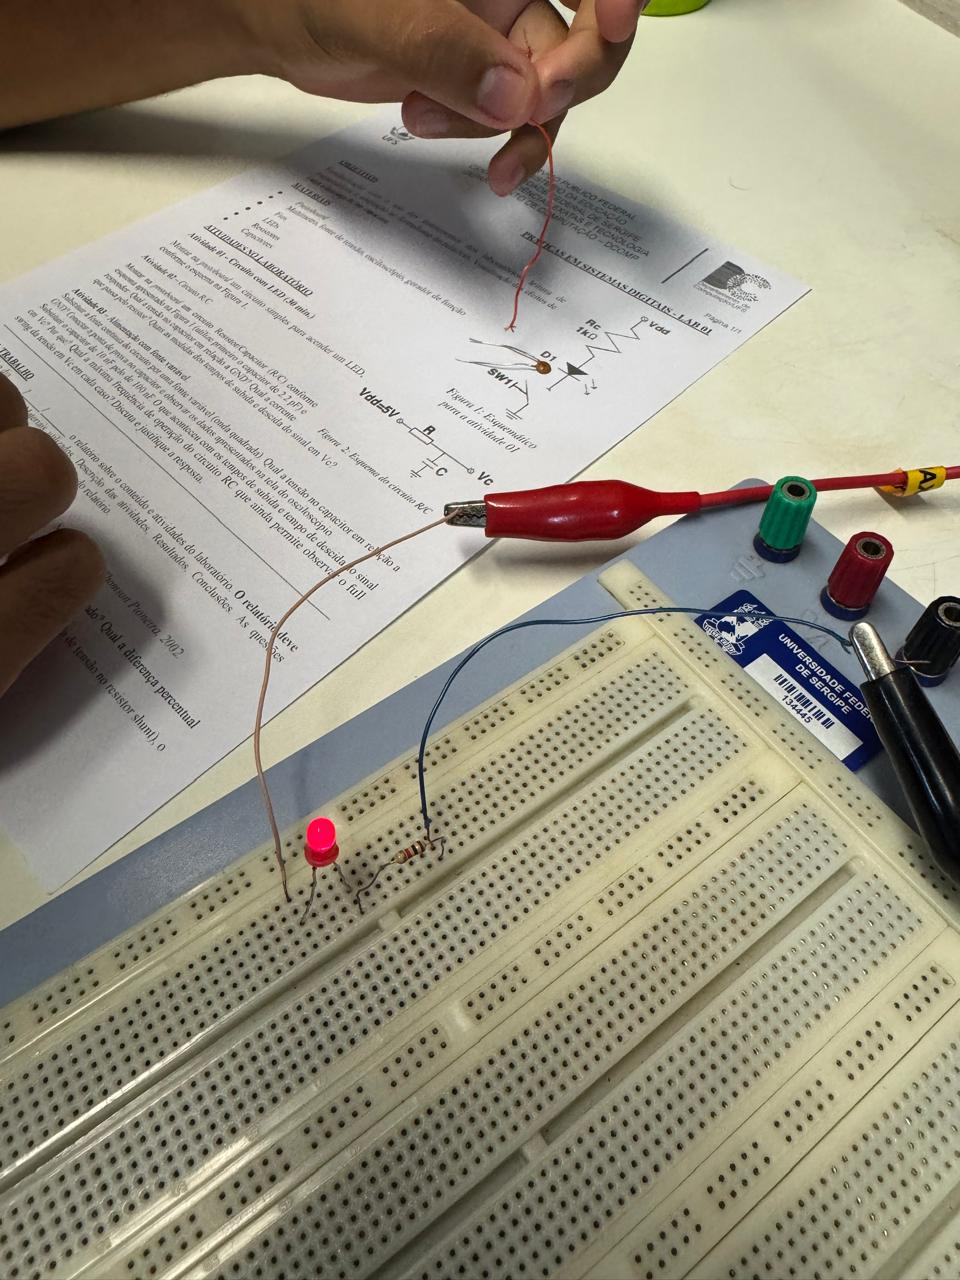
\includegraphics[width=0.7\columnwidth]{1.jpeg}}
\caption{Circuito básico montado em protoboard com o LED aceso.}
\label{fig1}
\end{figure}

\subsubsection{Circuito RC e Dinâmica Temporal}
Montou-se um circuito RC excitado por onda quadrada[cite: 1064]. Ao aumentar a capacitância para 100 nF, os tempos de transição subiram drasticamente[cite: 1065]. A tensão no capacitor obedece à constante $\tau = R \cdot C$; com capacitores maiores, a frequência máxima para observar o \textit{full swing} (transição total) diminui[cite: 1066, 1069]. A análise da corrente revelou picos pontuais apenas nos instantes de mudança de estado, análogo ao consumo dinâmico CMOS[cite: 1070, 1071].

\subsection{Conclusões do Laboratório 01}
A experimentação provou que transições lógicas não são instantâneas e que as capacitâncias governam os tempos de subida e descida[cite: 1073, 1074]. O desempenho de qualquer circuito digital é limitado pelo tempo físico de carga dos nós, justificando a dominância da tecnologia CMOS pelo seu baixo consumo estático[cite: 1075, 1076].

% ==========================================
% LABORATÓRIO 02
% ==========================================
\section{Laboratório 02: Famílias Lógicas e Inversores}

\subsection{Introdução Teórica}
A tecnologia TTL, baseada em transistores bipolares, foi o padrão inicial, mas foi substituída pela CMOS, que utiliza MOSFETs complementares[cite: 1084, 1086]. O CMOS suporta faixas de alimentação amplas e opera com alta impedância de entrada[cite: 1087]. A análise de \textit{datasheets} é obrigatória para verificar pinagens e limites elétricos[cite: 1088].

\subsection{Materiais Utilizados}
\begin{itemize}
    \item \textbf{Equipamentos:} Protoboard, multímetro, fonte contínua, fios e LEDs[cite: 1089].
    \item \textbf{CIs:} TTL 74LS04 (Inversor) e CMOS CD4007 (Transistores MOS discretos)[cite: 1090].
\end{itemize}

\subsection{Descrição das Atividades e Resultados}

\subsubsection{Características Típicas e Limites de Operação}
O TTL requer tensão fixa de 5V e possui margens estreitas de reconhecimento lógico[cite: 1092, 1093]. O CMOS tolera faixas de 3V a 15V, com limiares proporcionais a $V_{DD}$[cite: 1094]. As operações respeitaram esses limites para evitar danos térmicos[cite: 1095].

\subsubsection{Inversores TTL e CMOS}
Montou-se um inversor usando o 74LS04, comprovando que a saída é invertida em relação à entrada[cite: 1096, 1098]. Posteriormente, utilizou-se o CD4007 para construir o inversor de forma estrutural[cite: 1099]. A análise detalhada das formas de onda e das transições de estado foi efetuada através do osciloscópio, como mostra a Fig. 2.

\begin{figure}[htbp]
\centerline{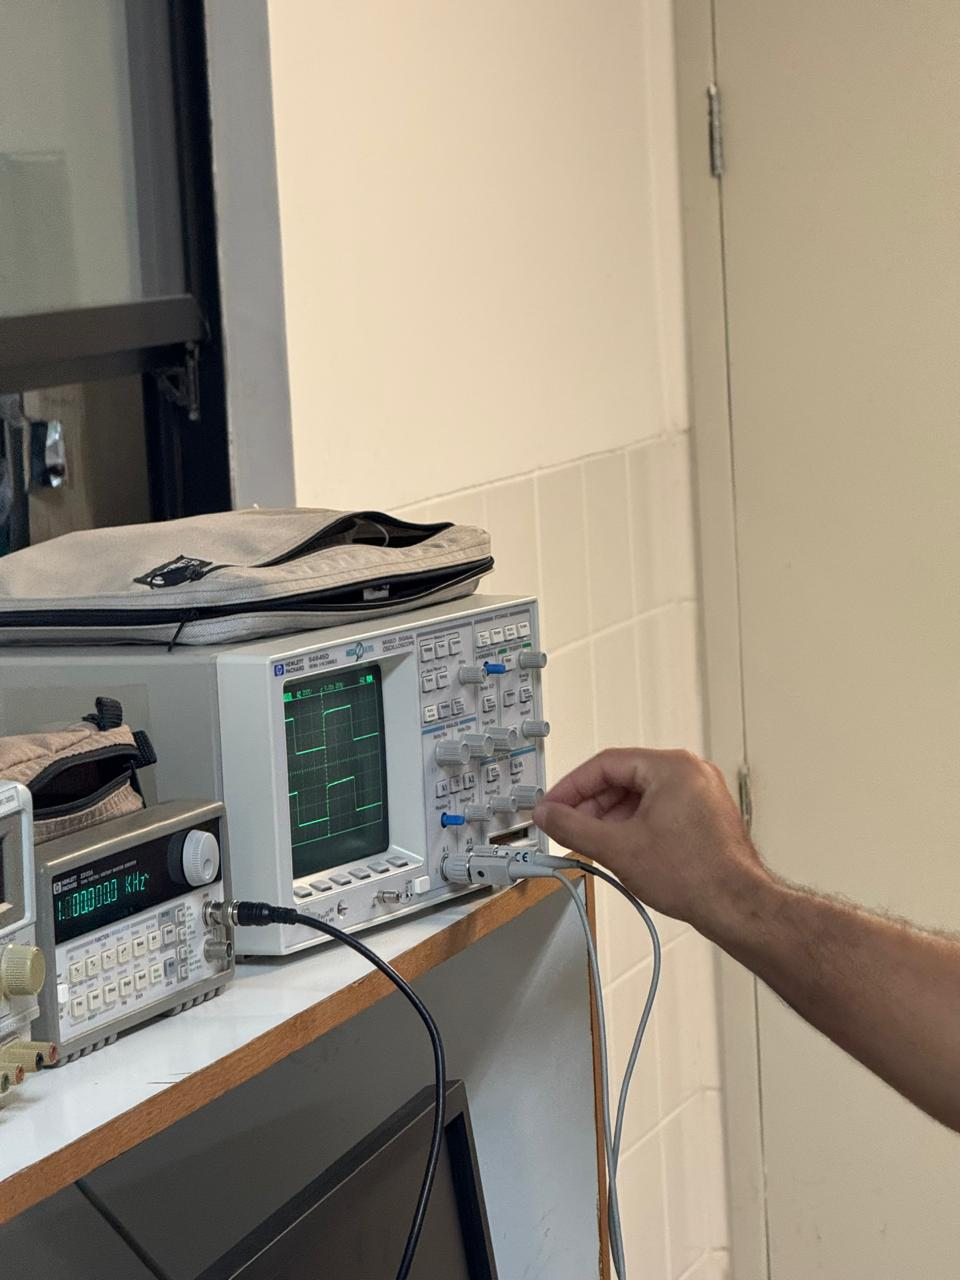
\includegraphics[width=0.7\columnwidth]{2.jpeg}}
\caption{Visualização das transições lógicas e níveis de tensão no osciloscópio.}
\label{fig2}
\end{figure}

\paragraph{Estrutura e Leiaute da Porta NOT CMOS}
A tecnologia CMOS utiliza menos componentes que a TTL[cite: 1100]. A montagem exigiu a união dos \textit{gates} para a entrada, a conexão da \textit{source} do PMOS ao $+V_{DD}$, da \textit{source} do NMOS ao GND, e a união dos drenos para a saída[cite: 1102, 1105].

\subsection{Conclusões do Laboratório 02}
Enquanto o TTL exige margens rigorosas de corrente, a topologia CMOS oferece consumo estático insignificante e flexibilidade de tensão[cite: 1107]. A montagem no CD4007 demonstrou a simplicidade geométrica da porta lógica, explicando a alta densidade de integração (VLSI) da tecnologia CMOS[cite: 1108, 1109].

\begin{thebibliography}{00}
\bibitem{b1} R. A. L. Reis, \textit{Concepção de Circuitos Integrados}. Porto Alegre: Bookman, 2009[cite: 1077, 1110].
\bibitem{b2} J. P. Uyemura, \textit{Sistemas digitais: uma abordagem integrada}. São Paulo: Thomson/Pioneira, 2002[cite: 1078, 1111].
\bibitem{b3} R. Tocci, N. Widmer, and G. Moss, \textit{Sistemas Digitais - Princípios e Aplicações}, 12. ed. São Paulo: Pearson, 2018[cite: 1079, 1112].
\end{thebibliography}

\end{document}